\documentclass{article}%
\usepackage[T1]{fontenc}%
\usepackage[utf8]{inputenc}%
\usepackage{lmodern}%
\usepackage{textcomp}%
\usepackage{lastpage}%
\usepackage[head=40pt,margin=0.5in,bottom=0.6in]{geometry}%
\usepackage{graphicx}%
%
\title{\textbf{Sustitutos que despiertan dudas}}%
\author{María Andreina Pernalete | mpernalete@el{-}nacional.com}%
\date{23/09/2018}%
%
\begin{document}%
\normalsize%
\maketitle%
\textbf{URL: }%
http://www.el{-}nacional.com/noticias/educacion/sustitutos{-}que{-}despiertan{-}dudas\_252826\newline%
%
\textbf{Periodico: }%
EN, %
ID: %
252826, %
Seccion: %
Educación\newline%
%
\textbf{Palabras Claves: }%
Investigación, Siete Días\newline%
%
\textbf{Derecho: }%
2.2, %
Otros Derechos: %
, %
Sub Derechos: %
2.2.1\newline%
%
\textbf{EP: }%
NO\newline%
\newline%
%
\textbf{\textit{}}%
\newline%
\newline%
%
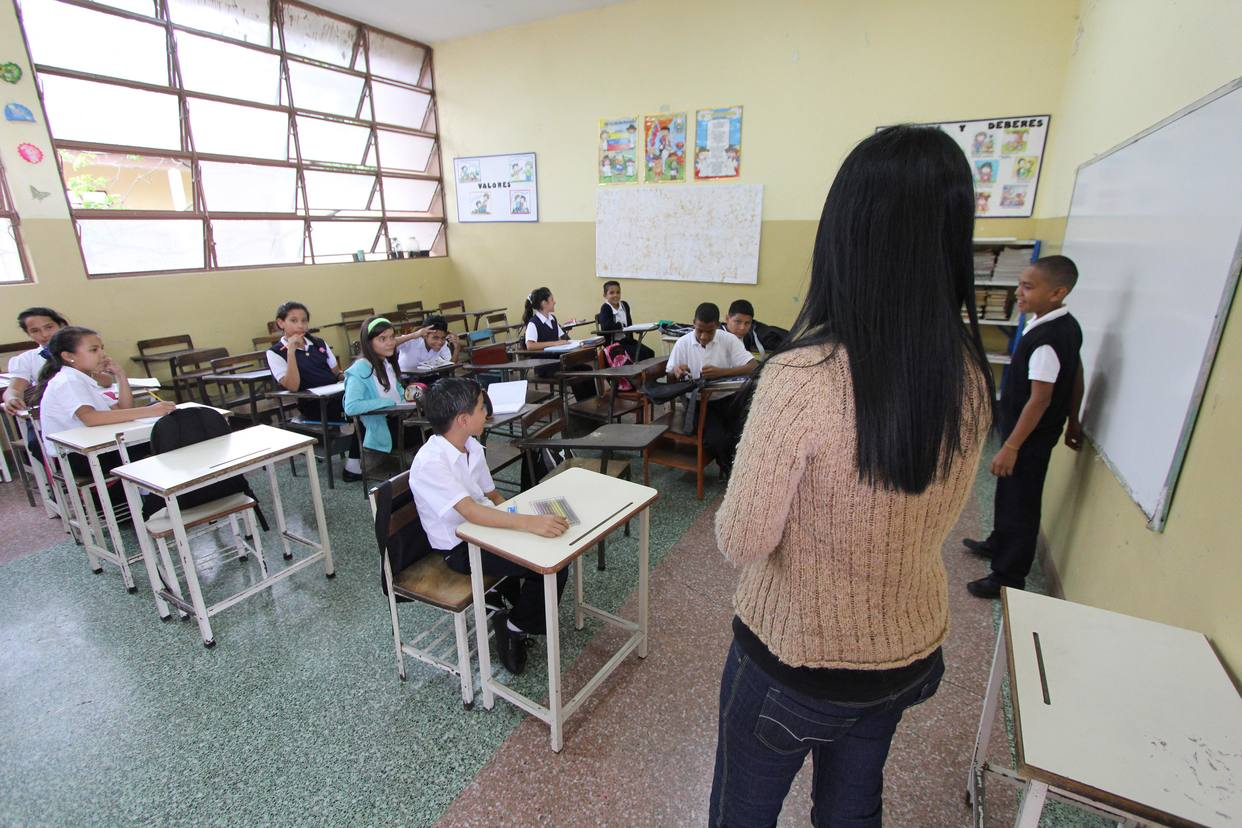
\includegraphics[width=300px]{79.jpg}%
\newline%
%
El regreso a clases comenzó con mal pronóstico: las escuelas son una muestra del vacío que ha dejado en el país la emigración de profesionales. Para llenar las vacantes de docentes, el gobierno ha ingresado en el sistema educativo a más de 9.600 participantes del Plan Chamba Juvenil. Especialistas reprueban la improvisación del programa y su evidente carga ideológica%
\newline%
%
Hasta hace seis meses Keimar Lucena, maestra egresada de Educación Especial, impartía clases en~la Unidad Educativa~Instituto Madre María, en Barquisimeto. Las dificultades económicas, los bajos sueldos y la escasez la hicieron sumarse al contingente de venezolanos que han emigrado. “Para nadie es un secreto la situación del país, y más la que afrontan los docentes”, dice. “Sin importar el tiempo de estudio y la~dedicación, el~maestro recibe un sueldo bajo, a diferencia de otros profesionales”.%
\newline%
%
Cuando emigró no pensó que encontrar trabajo sería tan fácil, pero a los dos días de haber llegado a Lima, donde está radicada, ya tenía cargo en un colegio como docente de educación inicial. Dice que hay días que está tranquila y contenta, pero otros en los que el recuerdo de sus estudiantes la invade. “Sí, extraño muchísimo a los niños de mi país”.%
\newline%
%
Los maestros también forman parte de los 2,3 millones de venezolanos que han dejado el país entre 2015 y 2017, según~la Organización Internacional~para las Migraciones. Esa ausencia se nota ahora en las aulas. Aunque no hay reconocimiento oficial del fenómeno, de manera indirecta fue aceptado por el Ministerio de Educación cuando anunció a mediados del año pasado que el Plan Chamba Juvenil, adoptado por el presidente Nicolás Maduro para ofrecer empleo a personas de entre 15 y 35 años de edad, también se dedicaría a subsanar el déficit de maestros en todo el país.%
\newline%
%
Un documento publicado en la web del~Centro Nacional para el Mejoramiento de~la Enseñanza~de las Ciencias~del Ministerio de Educación, organismo que asumió la tarea de incorporar a integrantes del Plan Chamba Juvenil en las escuelas, precisaba que en una primera etapa aspiraban a alistar a 10.000 participantes, que seguirían el Primer Curso Inicial para el Ingreso a~la Carrera Docente~con el propósito de “alcanzar una nueva institucionalidad educativa y garantizar la transición hacia una nueva sociedad”.%
\newline%
%
El curso de de 12 semanas que debían tomar los captados comprendería 5 módulos, con contenidos como reflexión sobre la identidad juvenil, formación sociopolítica y pedagogía popular “crítica y emancipadora”.%
\newline%
%
En esa primera etapa se informó que se había captado a 6.365 licenciados en educación, 197 graduados en espera de título de docente, 359 profesionales de otras áreas –como ingeniería y trabajo social– y 709 técnicos superiores universitarios, la mayoría en educación inicial e integral.%
\newline%
%
Sin embargo, Orlando Alzuru, presidente de~la Federación Venezolana~de Maestros, pone en duda las cifras oficiales: “Estamos seguros de que más de 80\% de los que entran a las escuelas por esa vía no tienen preparación para las aulas; se está haciendo un gran daño a la educación”.%
\newline%
%
El coordinador de~la ONG Memoria~Educativa de Venezuela, Luis Bravo Jáuregui, considera que en materia educativa el Plan Chamba Juvenil no es más que un nombre nuevo para una vieja pretensión. “Se trata de sustituir el trabajo profesional de educación por una labor ~amateur, por decirlo de alguna manera, lo que puede considerarse una agresión al equipo que se desempeña en los colegios”, dice.%
\newline%
%
Añade que es imposible evaluar la calidad del programa que sirve para formar a los maestros que se incorporan al sistema educativo, porque la información no ha sido publicada. “Eso despierta desconfianza acerca la preparación de esas personas”.%
\newline%
%
No obstante, Lenny Romero, presidente de Cenamec, defiende el perfil de los maestros procedentes del Plan Chamba Juvenil.~“De los chambistas~que ingresaron en un primer llamado, 311 desertaron por varias razones. Quedaron 9.605 que están dando clases en instituciones públicas. Solo 2\% no egresaron de Educación, pero todos son profesionales”, asegura.%
\newline%
%
Agrega que todos ellos tuvieron que tomar el curso de inducción, y los que no cuentan con título universitario como docentes están obligados a cursar la formación que imparte~la Micromisión SimónRodríguez, que requiere dos años de estudios. “La primera graduación sería en~2020”, aclara.%
\newline%
%
Pero la coordinadora del Observatorio Educativo de Venezuela, Olga Ramos, no cree que la formación que reciben esos integrantes del Plan Chamba Juvenil sea suficiente, porque no se imparte con el tiempo que se requiere; tampoco cubre los contenidos que ofrecería una formación universitaria completa.%
\newline%
%
Camino expreso.~El Plan Chamba Juvenil comenzó en junio de 2017. Un año después, el 20 de junio de 2018, Maduro le dio otro nombre, al bautizarlo como Gran Misión Socialista. Asimismo, se anunció que se le otorgaría “rango constitucional por medio de la asamblea nacional constituyente”, como señala la página oficial del Ministerio de~la Juventud~y el Deporte.%
\newline%
%
El presidente de~la Comisión~de~la Juventud~de~la ANC, Mervin Maldonado, afirmó el mismo día que esa instancia crearía la nueva ley “siguiendo las orientaciones del presidente”.~De acuerdo con la información oficial, más de 1 millón de jóvenes están inscritos en el sistema por medio del carnet de la patria y reciben un salario que representa 1.000 bolívares soberanos, más bonificaciones.%
\newline%
%
Ramos también rechaza la carga ideológica que rodea el programa de captación de maestros a través de la misión Plan Chamba Juvenil, lo cual parece confirmarse por la obligatoriedad de contar con el carnet de la patria para ser contratado.%
\newline%
%
Victoria García, nombre cambiado por motivos de seguridad, es una de las maestras que llegó a dar clases en una escuela pública a través de la ahora Misión Socialista. Es egresada de Educación Inicial de~la Universidad Bolivariana~de Venezuela y fue asignada a un colegio en Barquisimeto. “En junio de 2017 habilitaron el link y anunciaron que quien tuviera carnet de la patria y una carrera podía inscribirse, y yo lo hice. A las pocas semanas me llamaron directamente del Ministerio de Educación”, señala.%
\newline%
%
Tenía ocho años ejerciendo la carrera, pero no había podido ingresar a la nómina del ministerio. “Si no tienes palanca, no entras”, afirma. A pesar de que debió cumplir con el requisito de poseer carnet de la patria para que la contrataran, asegura que no pertenece a partido alguno; y al único que le agradece “es a Dios”, porque ahora tiene trabajo fijo. “En verdad nunca pensé que me llamarían; me inscribí por inscribirme”.%
\newline%
%
Da algunos detalles sobre el curso introductorio que debió seguir: “No dieron contenidos largos porque se supone que los asistentes deberían saber sobre los aspectos educativos. Sí hablaron acerca de cómo planificar las clases, pero las discusiones se basaron sobre todo en temas sociopolíticos”.%
\newline%
%
Perspectivas difíciles.~Ramos dice que es comprensible que en situaciones de urgencia se adopten medidas extremas para tratar de solventar los problemas. “En el caso de la educación es lícito que apeles a personas que no están formadas en el área, pero siempre deben contar con acompañamiento y tener acceso a material de calidad”, apunta.%
\newline%
%
Cita el ejemplo de una experiencia en~Colombia para garantizar la continuidad escolar en las escuelas multigrado (que concentran alumnos de varios niveles en un aula).~“Crearon~una estructura de escuelas en red: escuelas cabeceras y replicadoras. Las cabeceras tenían a los profesionales; las replicadoras contaban solo con quienes querían ayudar, pero también disponían de materiales y guías de trabajo con un diseño especialmente pensado para que el estudiante aprendiera”, indica Ramos. “Se trata de una práctica que podría funcionar en el caso venezolano”.%
\newline%
%
La especialista afirma que el Ministerio de Educación debería declararse en emergencia para tratar de afrontar la crisis y actuar en consecuencia con un programa bien estructurado, sin improvisar. Pero en lugar de eso parece evadir el problema del éxodo de profesionales. “Una cosa es lo que se dice oficialmente, y otra es la realidad”.%
\newline%
%
Romero admite que desconoce incluso si Aristóbulo Istúriz, nuevo ministro de Educación, continuará apelando a~la Misión Chamba~Juvenil.~“Todavía no se ha presentado un plan estratégico”, señala.~Pese a los evidentes problemas, entre ellos la migración masiva, el Ministerio de Educación sostiene que para el año escolar~2018{-}2019, que comenzó el 17 de septiembre, cuenta con~7.644.869 estudiantes en educación primaria, media, técnica y especial:~6.442.269~alumnos en planteles de educación oficial y 1.202.600 en colegios privados, lo cual significaría un aumento de 16,37\% con respecto al período 2017{-}2018.%
\newline%
%
Las consideraciones de Ramos adquieren mayor peso si se toma en cuenta que la crisis de la docencia parece empeorar, a propósito de las medidas económicas anunciadas recientemente. El 4 de septiembre, pocas semanas después de que entrara en vigencia la reconversión monetaria, comenzó a conocerse un nuevo tabulador salarial de la administración pública que no incluía a los docentes.%
\newline%
%
Bravo Jáuregui cree que las difíciles condiciones económicas constituyen un factor que empujará a más maestros fuera de las escuelas. “La decisión del gobierno de aplastar los salarios fue muy desmotivadora para los educadores”.%
\newline%
%
Oscar Meza, director del Centro de Documentación y Análisis Social de~la Federación Venezolana~de Maestros, comparte esa opinión. “El nuevo salario mínimo no logró compensar el poder adquisitivo, ni siquiera en su primer mes de vigencia”, asevera. “Así decreten que el salario de los docentes será el doble del actual, no tendrán capacidad para cubrir la canasta alimentaria”.%
\newline%
%
Cifras del Cendas esta semana indican que la canasta básica familiar se ubicó en agosto en 20.817 bolívares soberanos, mientras la canasta alimentaria llegó a más de 11.600 bolívares soberanos. Para quienes hacen vida en las escuelas, los problemas económicos vienen a sumarse a los de inseguridad, alimentación y ~transporte.%
\newline%
%
La presencia de educadores de~la Misión Chamba~Juvenil no es la única distorsión en el sistema educativo que preocupa a Ramos. “También ocurre que profesores de bachillerato están dando clases en primaria. Esto es gravísimo”, alerta. “No es lo mismo prepararse para atender niños que a jóvenes. Todos ellos tienen condiciones diferentes de aprendizaje”. Aunque la especialista señala que es lícito convocar a jubilados y a profesionales de otras áreas para resolver la ausencia de docentes, los primeros requieren de actualización profesional y los segundos de examen de conocimientos y cursos adecuados de capacitación.%
\newline%
%
El Estado, por otra parte, está obligado a dar seguimiento al trabajo en las instituciones y acompañar a los educadores desde el punto de vista psicológico y pedagógico, así como a evaluar su preparación por medio de exámenes de diagnóstico.%
\newline%
%
Romero asegura que en el caso de quienes son incorporados a las escuelas y no tienen formación docente, ofrecen acompañamiento a través de~la Micromisión Simón~Rodríguez: “Nuestras clases son de reflexión{-}acción, nosotros nos reunimos viernes y sábado para evaluar lo que se hace en las aulas”.%
\newline%
%
Alzuru también cuestiona los alcances de la micromisión Simón Rodríguez que, señala, ha sido un rotundo fracaso como alternativa del déficit de maestros. “La verdad es que hacer carrera como docente no está motivando a nadie por las graves dificultades económicas que atraviesa la profesión. La única manera de motivar a los maestros es ofrecer una remuneración atractiva”, manifiesta.%
\newline%
%
Ramos, sin embargo, hace énfasis en que se debe garantizar que esa formación cumpla con parámetros mínimos. “En educación no se ven los efectos de las deficiencias inmediatamente porque las personas no mueren si no aprenden a escribir, pero en el futuro las consecuencias pueden ser muy negativas. Quien no tiene competencias para buscar información, para analizar, para llegar a conclusiones, tiene truncadas sus opciones de vida”, advierte.%
\newline%
%
Añade que hay niños que requieren atención especial; y si los miembros de Chamba Juvenil no reciben ~asesoría idónea, podría ponerse en peligro su integridad. Sigue siendo necesario, reafirma, garantizar calidad educativa, con una planificación bien estructurada: “No se trata solo de llenar una ausencia”.%
\newline%
%
\end{document}